\section{Methodology}

\subsection{Data Cleaning and Preprocessing}

This study uses data from Crunchbase, a commercial database that has emerged as a primary source for entrepreneurship and venture‑capital research \cite{OECD2017}.  The platform contains detailed information on startups, investors and funding rounds.  Its data are collected through user submissions, web crawling and partnerships, supplemented by editorial curation \cite{OECD2017}.  Crunchbase provides comprehensive coverage of U.S. technology‑oriented transactions, making it well suited to studies of innovation ecosystems.

We queried Crunchbase for all investment transactions into enterprises domiciled in the United States and recorded all investors who participated in these rounds.  Foreign investors are included when they invest in U.S. companies.  Although Crunchbase has excellent coverage of technology‑driven ventures, several limitations and potential biases must be acknowledged \cite{OECD2017}:

\begin{itemize}
    \item \textbf{Geographic bias}: Stronger coverage of US and Western European markets compared to emerging economies.
    \item \textbf{Sectoral bias}: Emphasis on technology and internet companies, potentially underrepresenting traditional industries.
    \item \textbf{Venture capital bias}: Better documentation of VC-backed companies compared to bootstrapped or debt-financed ventures (which may not be problematic for this study).
    \item \textbf{Size bias}: Larger and more successful companies are more likely to be thoroughly documented.
    \item \textbf{Temporal bias}: More recent information tends to be more complete and accurate than historical records.
\end{itemize}

These biases do not invalidate research using Crunchbase but require careful consideration in study design and interpretation.  For network analysis of venture‑capital co‑investments, the VC bias may enhance data quality by focusing on the target population of interest.

The data preprocessing and cleaning follow established methodologies from entrepreneurship literature and network‑analysis practice \cite{Dalle2025}. After downloading the raw data, we performed the following steps:

\begin{enumerate}
    \item \textbf{Company data cleaning}: Removal of companies with incomplete essential information (missing unique identifiers, names, or founding years), exclusion of companies founded after 2017 to allow sufficient time for investment patterns to emerge, and removal of companies with exit status (closed, acquired, or IPO).
    
    \item \textbf{Investment data cleaning}: Removal of investment records with missing essential linkage information (company or investor identifiers), elimination of investments with invalid funding amounts (negative or zero values), and validation of funding consistency by excluding rounds where the sum of individual investments does not match the total funding amount reported in the database.
    
\item \textbf{Funding threshold}: Restrict the sample to companies that raised more than \$150{,}000 in total funding to focus on substantive investment relationships and ensure statistical reliability.
    
    % \item \textbf{Endogeneity bias prevention}: Exclusion of companies that received funding exclusively from accelerators or incubators to prevent endogeneity bias, as these companies may not have attracted independent market validation from external investors.
    
    \item \textbf{Data consistency validation}: Final consistency checks to ensure all investment records reference existing companies in the dataset and all retained companies have at least one valid investment record.
\end{enumerate}

\subsection{Network Construction}

The network construction process transforms the cleaned investment data into a structured bipartite representation. Rather than projecting a one‑mode investor–investor network, we model the system as a bipartite graph connecting early‑stage investors to late‑stage investors through their shared portfolio companies.  This approach captures both the sequential flow of capital across funding stages and the solidarity of syndication partnerships.  It follows the conceptual distinction between flow and bond models in social‑network analysis \cite{Borgatti2009}. 

A one‑mode projection would obscure stage‑specific roles and over‑estimate connectivity; the bipartite structure retains the heterogeneity of investor types and allows us to study how early and late investors are coupled through co‑investment.

The construction process involves three sequential transformations, each representing a different conceptualization of network ties, each one described in \ref{fig:bipartite_pipeline} and in the subsequent paragraphs below.

\begin{figure}[htbp]
    \centering
    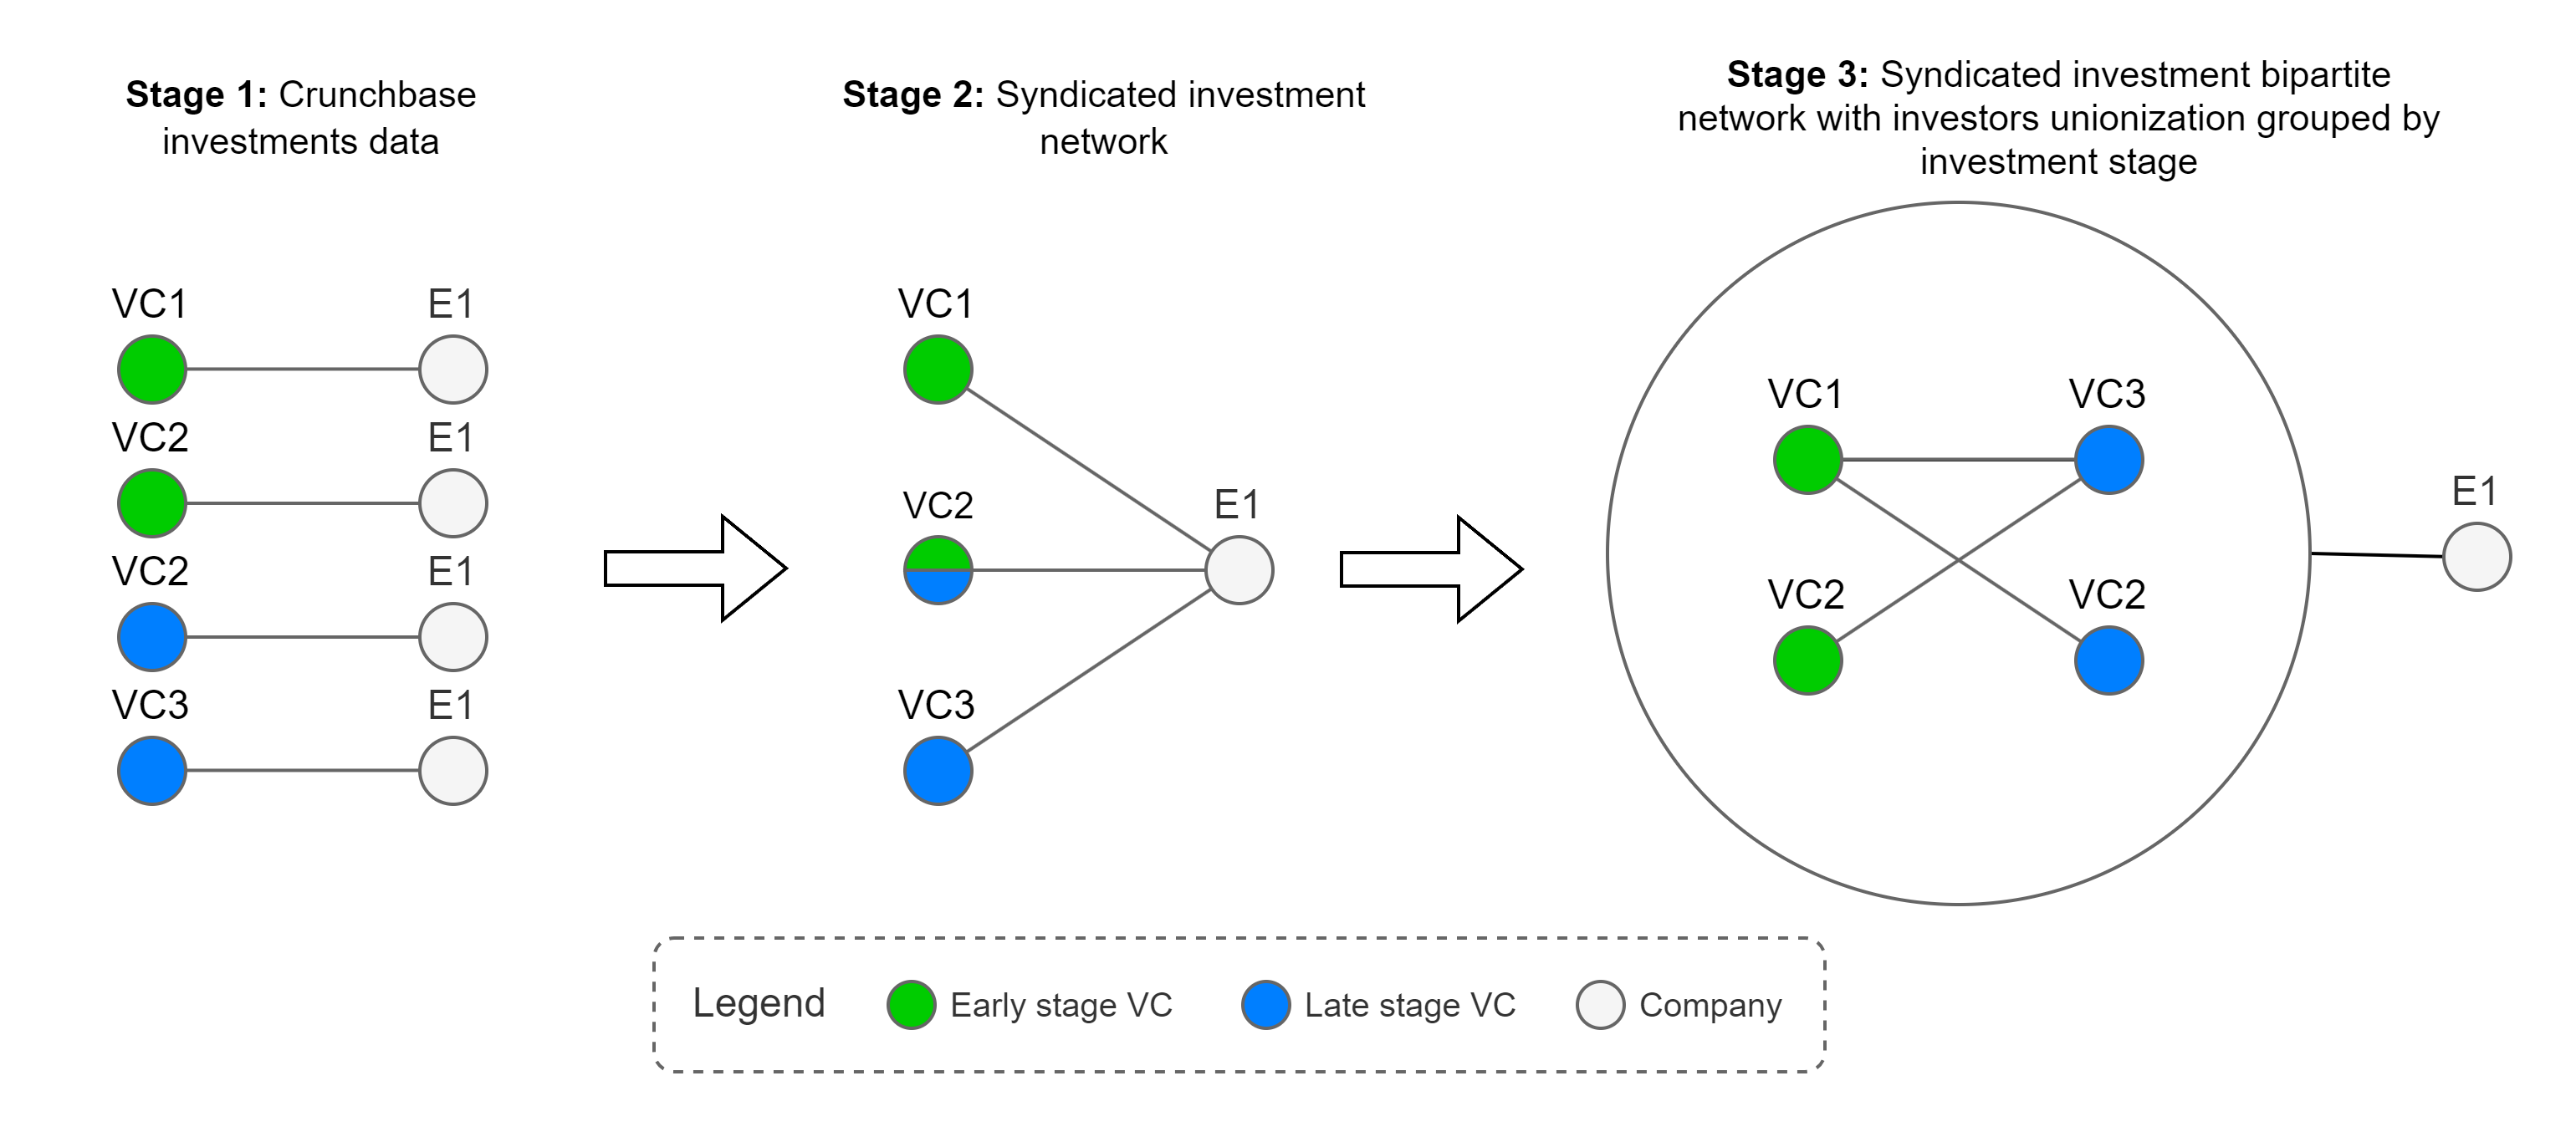
\includegraphics[width=\textwidth]{../diagrams/vc_investment_bipartite_pipeline.png}
    \caption{Pipeline from event-level records to the bipartite syndication network linking late- to early-stage investors.}
    \label{fig:bipartite_pipeline}
\end{figure}

\textbf{Stage~1 – Raw event‑type investment ties:}
The initial Crunchbase dataset records discrete transactional relationships between venture‑capital firms and portfolio companies.  These event‑type ties represent what \cite{Borgatti2009} characterise as nominalist network constructions: the investment transaction is the fundamental tie type at this stage.  Each investment event creates a direct dyadic relationship between a venture‑capital firm and a company, but these isolated ties do not yet reveal broader co‑investment patterns.

\textbf{Stage~2 – Syndicated investment network construction:}
The raw event data are aggregated to identify co‑investment relationships, where multiple venture‑capital firms participate in the same funding round or invest in the same company across different rounds.  This aggregation transforms discrete events into a network structure in which venture‑capital firms become indirectly connected through their shared ties to portfolio companies.  Following \cite{Borgatti2009}, this step creates pathways between actors that enable analysis of their relative positions, including measures of centrality and brokerage within the investment ecosystem.

\textbf{Stage 3 - Bipartite network segmentation by investment stage:}
The final transformation reorganizes the syndicated network into a bipartite structure that separates investors based on their participation in different funding stages. 

First, investment stages are categorized into two main groups:
\begin{itemize}
    \item Early stages: angel, pre-seed, seed, and Series A
    \item Late stages: Series B through Series I
\end{itemize}

This bipartite structure simultaneously reflects flow and bond models \cite{Borgatti2009}.  From a flow perspective, it allows us to analyse how resources and information traverse funding stages; from a bond perspective, it captures the cohesion of co‑investor coalitions within each stage.  Modelling both perspectives explicitly is essential because early–stage and late–stage investors perform distinct roles in syndication.

An important consideration in this construction involves investors who participate in both early and late stages (for example, a venture capital firm that invests in both Series A and Series C rounds). In such exceptional cases, the same investor appears as distinct agents on both sides of the bipartite network. 

This separation is achieved by appending the investment stage identifier to the unique investor UUID during the network construction process, effectively creating stage-specific identities for multi-stage investors. This approach ensures that the bipartite structure remains mathematically valid while preserving the analytical ability to study how the same investor behaves differently across investment stages.

The resulting bipartite graph connects two distinct sets of investors: those participating in early-stage rounds and those participating in late-stage rounds. Edges represent co-investment relationships where early-stage and late-stage investors have both invested in the same company, creating a bridge between different phases of the venture capital investment cycle.

Formally, the bipartite graph $G = (U \cup V, E)$ consists of:
\begin{align}
U &= \{u_1, u_2, \ldots, u_m\} \text{ (late-stage VCs)} \\
V &= \{v_1, v_2, \ldots, v_n\} \text{ (early-stage VCs)} \\
E &\subseteq U \times V \text{ (co-investment relationships)}
\end{align}

To prevent spurious connections from related entities, investor pairs where the first five characters of their names match are filtered out, reducing the likelihood of including different funds from the same parent organization (even though it does not change our results as per numerous experiments). Furthermore, investors that participated in both early and late stages receive a suffix so they can be treated as distinct agents for each phase.

\subsection{Community Detection}

Community structure in the bipartite network is identified using modularity optimisation.  Modularity was introduced by Newman as a measure of the excess density of edges within communities compared with a random null model \cite{Newman2003}.  For bipartite graphs, Barber \cite{Barber2007} proposed an adjusted modularity function that accounts for the two disjoint node sets.  We adopt a greedy optimisation algorithm that iteratively merges communities to maximise this bipartite modularity. 

Greedy heuristics have proved effective at uncovering meaningful structure while scaling to large graphs \cite{Blondel2008}. Although more advanced methods such as the Leiden algorithm offer improvements in connectivity \cite{Traag2019}, we verified that applying Leiden to a subset of the data yielded similar community assignments. This robustness check suggests that our results are not an artefact of algorithm choice.

For a bipartite network, the modularity $Q$ is defined as:
\begin{equation}
Q = \frac{1}{2m} \sum_{i,j} \left[ A_{ij} - \frac{k_i k_j}{2m} \right] \delta(c_i, c_j)
\end{equation}

where $A_{ij}$ is the adjacency matrix, $k_i$ is the degree of node $i$, $m$ is the total number of edges, $c_i$ is the community of node $i$, and $\delta(c_i, c_j)$ is 1 if nodes $i$ and $j$ are in the same community, 0 otherwise.

To test the stability of our findings, we repeated the community‑detection procedure under multiple random seeds and compared the resulting partitions.  We also performed a sensitivity analysis using the Leiden algorithm \cite{Traag2019}.  In all cases, the three largest communities remained almost identical in composition and size.  This robustness gives confidence that our findings are not sensitive to algorithmic or stochastic variation.

Modularity‑based community detection has proven effective in venture‑capital research.  Bubna et~al.\ showed that modularity optimisation on co‑investment networks uncovers persistent communities with distinct investment strategies \cite{Bubna2020}.  We build on this basis to explore structural patterns that go beyond degree distributions.

\subsection{Nestedness Analysis}

Nestedness is a structural property observed in ecological networks \cite{Bascompte2003,AlmeidaNeto2008} that describes the tendency for specialists to interact with subsets of the partners of generalists.  In the context of venture‑capital syndication, nestedness would mean that investors with few ties tend to co‑invest with a subset of the partners of highly connected investors.

We measure nestedness using the NODF (Nestedness based on Overlap and Decreasing Fill) metric \cite{AlmeidaNeto2008}.  NODF has become a standard measure for quantifying nested patterns in bipartite networks; it accounts for both the overlap of connections and the degree differences between nodes \cite{Dormann2009}.  A perfect nested structure yields $\mathrm{NODF}=1$, while a random structure yields values close to zero.

For a bipartite adjacency matrix $M$ with rows and columns sorted by decreasing degree, NODF is calculated as:

\begin{equation}
NODF = \frac{NODF_{rows} + NODF_{columns}}{2}
\end{equation}

where:
\begin{align}
NODF_{rows} &= \frac{100}{R(R-1)/2} \sum_{i=1}^{R-1} \sum_{j=i+1}^{R} \frac{|N_i \cap N_j|}{k_j} \text{ if } k_i > k_j \\
NODF_{columns} &= \frac{100}{C(C-1)/2} \sum_{i=1}^{C-1} \sum_{j=i+1}^{C} \frac{|N_i \cap N_j|}{k_j} \text{ if } k_i > k_j
\end{align}

Here, $R$ and $C$ are the number of rows and columns, $N_i$ represents the set of connections for node $i$, and $k_i$ is the degree of node $i$.

Using this method, NODF values range between 0 and~1 (perfect nestedness).

\subsection{Statistical Significance Testing}

To determine whether observed nestedness values differ significantly from what would be expected by chance, we employ a null‑model approach using the Curveball algorithm \cite{Strona2014}.  Curveball generates randomized matrices that preserve the degree sequence of both node sets while randomising the connection patterns.  

Preserving the degree sequence is critical because degree heterogeneity alone can induce apparent nestedness; a degree‑preserving null model allows us to test whether the observed hierarchical organisation goes beyond what could arise from simple degree sequences \cite{Ulrich2007,Dormann2009}.

For each community we generate 1{,}000 null matrices using 10{,}000 Curveball iterations.  Increasing the number of null matrices improves the precision of the p‐value estimates at the cost of higher computational time.  We verified that results were qualitatively unchanged when using 500 or 2{,}000 null matrices.

For each community, we compute the mean ($\mu_{\mathrm{null}}$) and standard deviation ($\sigma_{\mathrm{null}}$) of the null NODF values.  We then calculate a standardized Z‑score to quantify how many standard deviations the observed nestedness differs from the null expectation:

\begin{equation}
Z = \frac{NODF_{observed} - \mu_{null}}{\sigma_{null}}
\end{equation}

where $\mu_{null}$ and $\sigma_{null}$ are the mean and standard deviation of the null distribution, respectively.

The empirical p‑value is calculated as the proportion of randomised matrices that exhibit nestedness equal to or greater than the observed value:

\begin{equation}
p = \frac{1 + \sum_{i=1}^{N} I(NODF_{null,i} \geq NODF_{observed})}{N + 1}
\end{equation}

where $N$ is the number of null matrices, $NODF_{\mathrm{null},i}$ is the nestedness score of the $i$‑th null matrix and $I(\cdot)$ is an indicator function equal to 1 when the condition is true and 0 otherwise.  Adding 1 to the numerator and denominator yields a conservative p‑value estimate and avoids values of exactly zero.

The p‑value represents the probability of observing nestedness as high as or higher than the observed value under the null hypothesis of random co‑investment patterns.  Communities with $p<0.05$ are considered to have significantly high nestedness (when the observed value exceeds the null expectation) or significantly low nestedness (when the observed value falls below it).

Z‑scores and p‑values provide complementary information: the Z‑score quantifies how many standard deviations the observation lies from the null mean, whereas the p‑value gives the tail probability.

As an additional robustness check we repeated the null‑model analysis across multiple random seeds and confirmed that the significance outcomes were stable.  We also varied the threshold for community size (150 investors) and found that the qualitative conclusions about which communities exhibited significant nestedness remained unchanged.

\pagebreak